\section{Merging Obfuscation Specialists}
\label{sec:merging}

We train low-rank adapters independently on different program
representations and compose the resulting specialists into a single adapter
before inference. The default merge contains six adapters: one clean-code
specialist, \texttt{L0}, and five obfuscation specialists,
\texttt{L1b}, \texttt{L1r}, \texttt{L2}, \texttt{S1}, and \texttt{S2}.
Each specialist is optimized independently while the base model remains
frozen. After training, the specialists are merged once offline and the
individual adapters are discarded.


Figure~\ref{fig:merge_pipeline} summarizes the complete procedure. Each
condition produces an independently trained LoRA specialist; corresponding
adapter parameters are then composed offline using DARE-TIES, yielding a
single adapter that is deployed without routing or an expert bank.



\begin{figure}
    \centering
    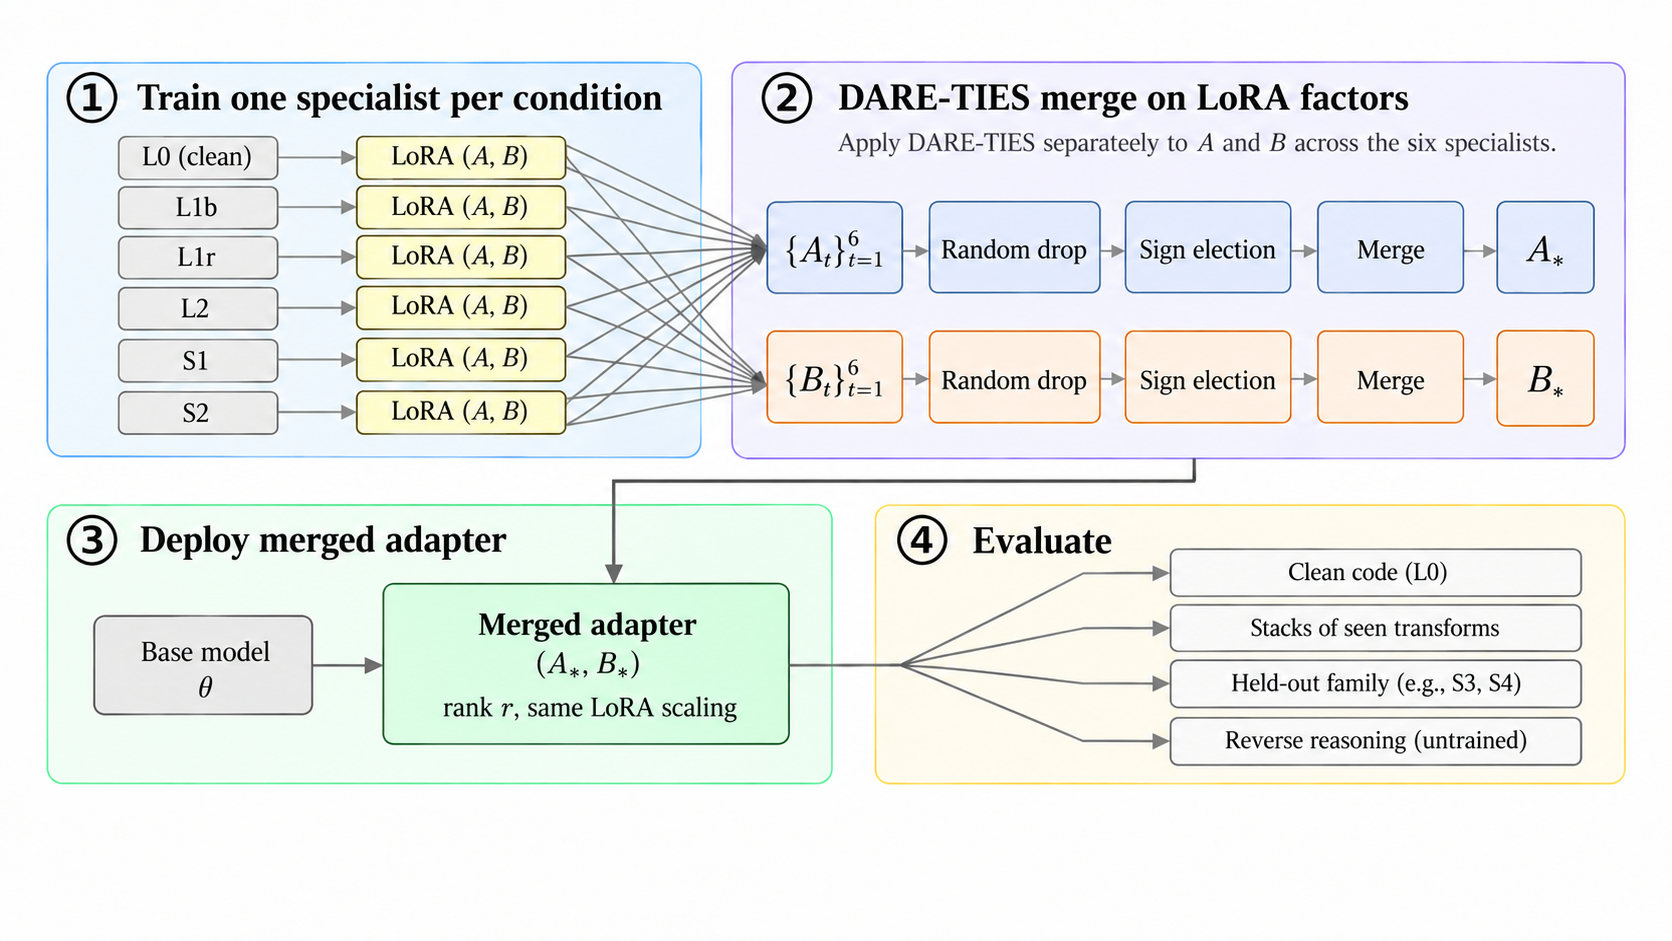
\includegraphics[width=1\linewidth]{figures/pipeline_fig.png}
\caption{\textbf{Overview of our methodology.}
We train six LoRA specialists: one on clean code (\texttt{L0}) and five on
seen obfuscations (\texttt{L1b}, \texttt{L1r}, \texttt{L2}, \texttt{S1},
and \texttt{S2}). We merge the corresponding $A$ and $B$ factors separately
with DARE-TIES to obtain a single adapter, which is deployed without a router
or expert bank and evaluated across clean, stacked, held-out, and
reverse-reasoning conditions.}
\label{fig:merge_pipeline}
\end{figure}



This separates \emph{specialization} from \emph{composition}. Each adapter
learns from a single transformation condition without jointly optimizing
against examples from the other conditions. Composition then occurs only after
specialist training, producing one adapter with the same inference-time
architecture as an ordinary LoRA model. Unlike routing, the deployed model
requires neither a gate nor a resident bank of specialists.

Let the frozen base parameters be $\theta$, and let
$\Delta\theta_t$ denote the low-rank update learned by specialist $t$.
Independent training produces

\[
\{\Delta\theta_1,\ldots,\Delta\theta_T\}.
\]

We compose these updates using a parameter-space merge operator
$\mathcal{M}$,

\[
\Delta\theta_{\mathrm{merge}}
=
\mathcal{M}
\left(
\Delta\theta_1,\ldots,\Delta\theta_T
\right),
\]

and deploy

\[
\theta'
=
\theta + \Delta\theta_{\mathrm{merge}}.
\]

\paragraph{LoRA representation.}
For an adapted weight matrix $W$, specialist $t$ represents its update as

\[
\Delta W_t = B_t A_t,
\]

where $A_t$ and $B_t$ are rank-$r$ LoRA factors. All specialists use the
same rank, scaling coefficient, and target modules, so corresponding adapter
parameters can be merged directly across specialists. The resulting merged
adapter has the same rank and target modules as the individual specialists.

\paragraph{Merge operator.}
We evaluate TIES and DARE-TIES merging. All specialists receive uniform merge
weights. TIES first removes low-magnitude parameter changes, determines a
consensus sign for each retained coordinate, and averages only updates that
agree with that sign. DARE-TIES applies random sparsification and rescaling to
the task-specific parameter updates before the TIES sign-resolution and
aggregation step. We use a retained density of $0.5$ for all models.

The density is fixed across the eight evaluation models. It was selected from
$\{0.3,0.5,0.7\}$ using a separate 1.5B-parameter pilot model and was not tuned
on the reported model panel. Unless otherwise stated, the main results use
DARE-TIES; TIES is reported as a merge ablation.

% VERIFY THIS SENTENCE AGAINST THE IMPLEMENTATION:
The merge is applied independently to corresponding LoRA parameter tensors at
each adapted layer, rather than materializing and merging the full base-model
weights.


\paragraph{The operator is not arbitrary.} Sparsification and sign election, rather than averaging,
do most of the work. Rebuilding the merge with plain uniform averaging at identical ingredients,
weights, density, rank and seed (Table~\ref{tab:mergeop}) does not merely lose: on three of four
models it does not clear the format gate on clean code or on the seen single transforms at all, and
on the one unseen-family cell where it is readable it reaches $25\,\%$ of the untuned model's
clean-code accuracy against an untuned baseline of $57\,\%$ --- worse than not merging. Averaging is
also the only operator that loses the answer contract: it answers the forward question when asked to
reverse on $0.174$ and $0.428$ of items on the two models read in that direction, where TIES sits at
$0.000$ and DARE-TIES at $0.019$ and $0.000$. Three operators at one density is not a search, so we
do not claim DARE-TIES is optimal, only that the choice is load-bearing.

% GENERATED by scripts/analysis/82_merge_operator.py -- do not edit by hand.
\begin{table}[t]
\centering\small\setlength{\tabcolsep}{5pt}
\caption{\textbf{The merge operator is not arbitrary.} Forward accuracy as a percentage of the untuned model's clean-code accuracy on the same programs. Ingredients, weights, density, rank and seed are identical across the three merges; only the operator differs. \emph{linear} is plain uniform averaging, with no sparsification and no sign election. \textbf{Averaging does not merely lose, it breaks the answer contract}: where it is readable at all it recovers little more than not merging, and it is the only operator with a non-zero direction-lock rate (\emph{lock}: the fraction of backward replies that are the gold \emph{forward} answer). \texttt{gated}: every cell of that arm exceeded the 0.25 format-failure gate. \texttt{--}: not run --- backward and lock were read on two models only, the other two having been cancelled to stay inside a 15-GPU cap once the forward answer was unambiguous on four.}
\label{tab:mergeop}
\begin{tabular}{@{}llrrrr@{}}
\toprule
model & operator & \texttt{L0} & singles & unseen & lock \\
\midrule
CodeLlama-7B & \emph{base} & 100 & 75 & 46 & 0.000 \\
 & \textsc{linear} & \texttt{gated} & \texttt{gated} & \texttt{gated} & 0.174 \\
 & \textsc{ties} & 142 & 124 & 88 & 0.000 \\
 & \textsc{dare-ties} & 164 & 147 & 105 & 0.019 \\
\addlinespace[2pt]
CodeLlama-13B & \emph{base} & 100 & 85 & 57 & \texttt{--} \\
 & \textsc{linear} & \texttt{gated} & \texttt{gated} & 25 & \texttt{--} \\
 & \textsc{ties} & 163 & 143 & 95 & \texttt{--} \\
 & \textsc{dare-ties} & 188 & 168 & 120 & \texttt{--} \\
\addlinespace[2pt]
Llama-3.1-8B & \emph{base} & 100 & 85 & 52 & 0.000 \\
 & \textsc{linear} & 115 & 98 & \texttt{gated} & 0.428 \\
 & \textsc{ties} & 154 & 133 & 83 & 0.000 \\
 & \textsc{dare-ties} & 178 & 156 & 104 & 0.000 \\
\addlinespace[2pt]
Granite-3.1-8B & \emph{base} & 100 & 92 & 58 & \texttt{--} \\
 & \textsc{linear} & \texttt{gated} & \texttt{gated} & \texttt{gated} & \texttt{--} \\
 & \textsc{ties} & 133 & 119 & 72 & \texttt{--} \\
 & \textsc{dare-ties} & 152 & 132 & 82 & \texttt{--} \\
\bottomrule
\end{tabular}
\end{table}


\paragraph{Training and deployment.}
Specialists are trained independently using the same optimization setup and
base checkpoint. Merging is performed only after specialist training and
requires no additional optimization. No transform identity, routing decision,
or dynamic expert selection is used during evaluation. Consequently, the
deployed artifact is a single low-rank adapter and has the same inference-time
parameterization and computational structure as the other single-adapter
baselines.